\section{Method}

The experimental setup is shown in figure \ref{fig:setup}.

Uncertainties are carried through calculations via uncertainty propogation, following:
\begin{equation}
    \label{eq:uncertainty}
    \delta f = \sqrt{\left(\frac{\partial f}{\partial x}\delta x\right)^2 + \left(\frac{\partial f}{\partial y}\delta y\right)^2 + \ldots}
\end{equation}

\begin{figure}[H]
    \centering
    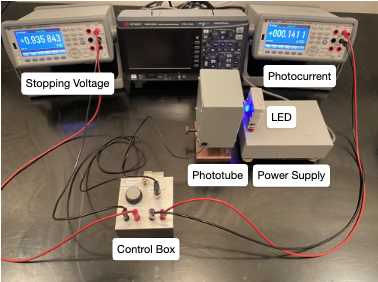
\includegraphics[width=0.8\textwidth]{method/setup.png}
    \caption{Experimental setup}
    \label{fig:setup}
\end{figure}

The light source consists of interchangeable LEDs of different frequencies. A control box allows us to change the applied reverse voltage, which will be used to obtain the stopping current.
The control box also allows the measurement of the photocurrent as a voltage across a 100 $K\Omega$ resistor. The voltage is then measured with the multimeter.

\subsection{Part 1: Planck's Constant and Work Function}

In this section we will measure the stopping voltage for different wavelengths (by using the different LEDs provided for the experiment) of light using the stopping voltage multimeter, as shown in Figure \ref{fig:setup}.
The stopping voltage is the voltage required to stop the electrons from reaching the anode.
The stopping voltage is proportional to the frequency of the light, and the proportionality constant is Planck's constant according to equation \ref{eq:stopping}.

Based on the values, we obtain Planck's constant, the work function for the phototube, as well as the cutout frequency for the phototube by fitting the data to a linear regression model.

\subsection{Part 2: Stopping voltage and photocurrent as a function of intensity}

In this section we will measure the stopping voltage and photocurrent as a function of the intensity of the incident light using both the stopping voltage and photocurrent multimeters,
and the potentiometer LED to change the intensity of the light.

This will help us gain insight into the differences between the original and Einstein's model of the photoelectric effect.

\subsection{Part 3: Photocurrent delay}

In the last section of the report, we make use of the provided osciloscope to generate a periodic signal that will be used to
measure the time delay between the light being turned on and the current reaching a steady state.

The photocurrent will also be examined using the osciloscope, and compared directly to the signal generated.


This will help us understand the time it takes for the electrons to be emitted from the material to draw conclusions about different explanations of the photoelectric effect.
